\chapter{Experiments}\label{c:experiments}

Precision and recall are favoured values in image retrieval. Precision is the fraction of the number of relevant retrieved objects and the number of all the retrieved objects. Recall is the ratio of the number of relevant retrieved objects to the number of all the relevant objects. Although, many retrieval systems are capable to return a ranked list of the retrieved objects, precision and recall ignore this information. Thus, the trained models are evaluated with the nowadays very popular mean average precision (mAP) metric.
\bigbreak
All the mentioned results are then calculated with the evaluation implementation of py-faster-R-CNN \cite{Girshick2017} \cite{NIPS2015_5638}. Firstly, it creates a descending sorted list for every company (class), based on the probabilities of being logos from the specific brand on given positions of the images. Then, the precision curve, as a function of recall, is acquired for every list. The average precision is then calculated as the area under the curve. The average of these values gives the mean average precision.
\bigbreak
The models trained for logo detection are evaluated beside of mAP, with free-response receiver operating characteristic (FROC) curve \cite{MillerTheFROC1969}. This metric was first used for cancer localization in medical images. On this curve the detection rate aka. recall (the fraction of the number of the true positive detections and the number of all the positive locations in the dataset) is plotted over the average number of false detections per image. Since the detectors should be optimized to have a recall, as high as possible, this curve gives an intuitive interpretation about the performance of a detector.
\bigbreak
If not stated otherwise, all the models are trained for 80k iterations with a base learning rate of 0.001, which is reduced to its one-tenth after every 50k iterations. All the training and testing are performed in Caffe deep learning framework \cite{Jia:2014:CCA:2647868.2654889}.
\bigbreak
\section{Training with Synthetic Data}
In this section, the effect of synthetic data to the logo detection performance will be examined. For this purpose, the detector was trained on existing and generated datasets.

Synthetic data was already used to test its impact to logo retrieval by \cite{DBLP:journals/corr/SuZG16}. However, they reported the performance improvements, by extending a very scarce real training data with synthetic data (10 training images of FL-32 pro class). It is questionable whether the synthetic images would have helped so much if more real training data had been used (e.g. 40 images pro class, by using the validation set of FL-32 too).
\bigbreak
\subsection{FlickrBelgaLogos dataset}\label{ss:flickrbelgalogos}

A dataset, which is annotated manually, may contain logos, which stay unannotated. If a system is evaluated on such a dataset, and detects the unannotated logo, it counts as false positive. Thus, a synthetic dataset, called FlickrBelgalogos \cite{letessier2012scalable} is created for evaluation purpose by pasting the logo annotations of the dataset BelgaLogos \cite{belgalogos09} on images from Flickr to random positions. One could argue with the correctness of evaluating a detector with this dataset, because alone the contrast difference may make the logos easier to detect on these images.

\begin{figure}
  \centering
\begin{tabular}{cccc}
  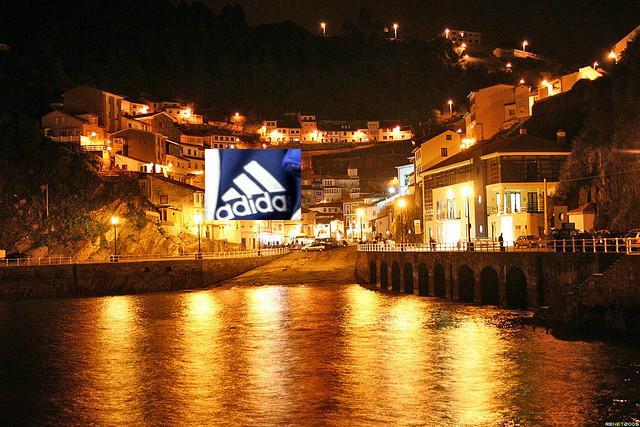
\includegraphics[width=25mm]{images/mt/flbl1.jpg} &   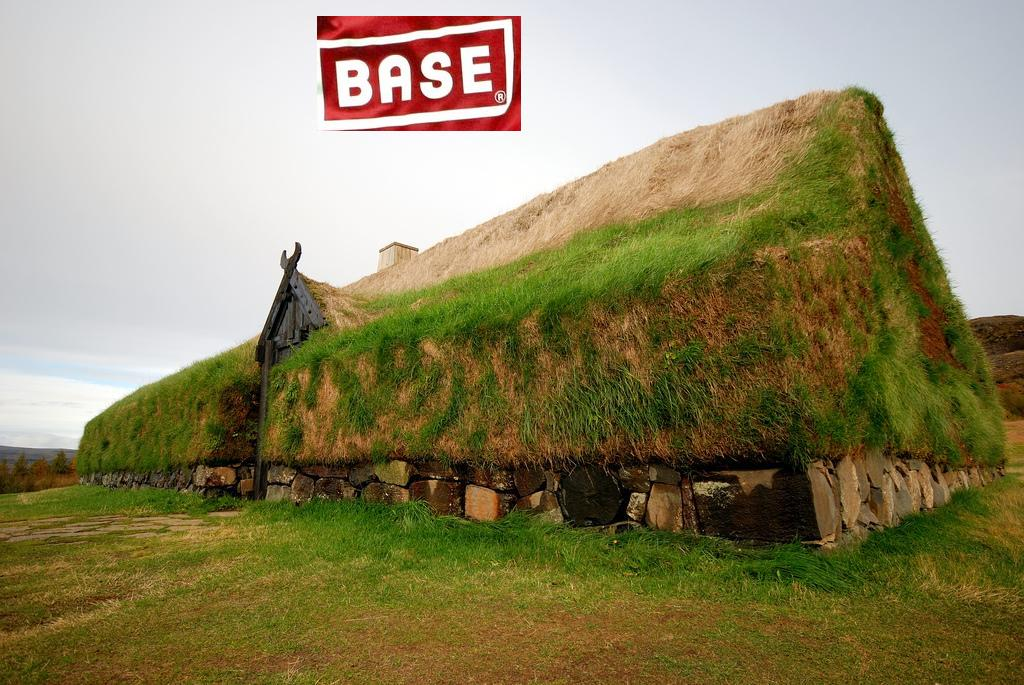
\includegraphics[width=25mm]{images/mt/flbl2.jpg}  & 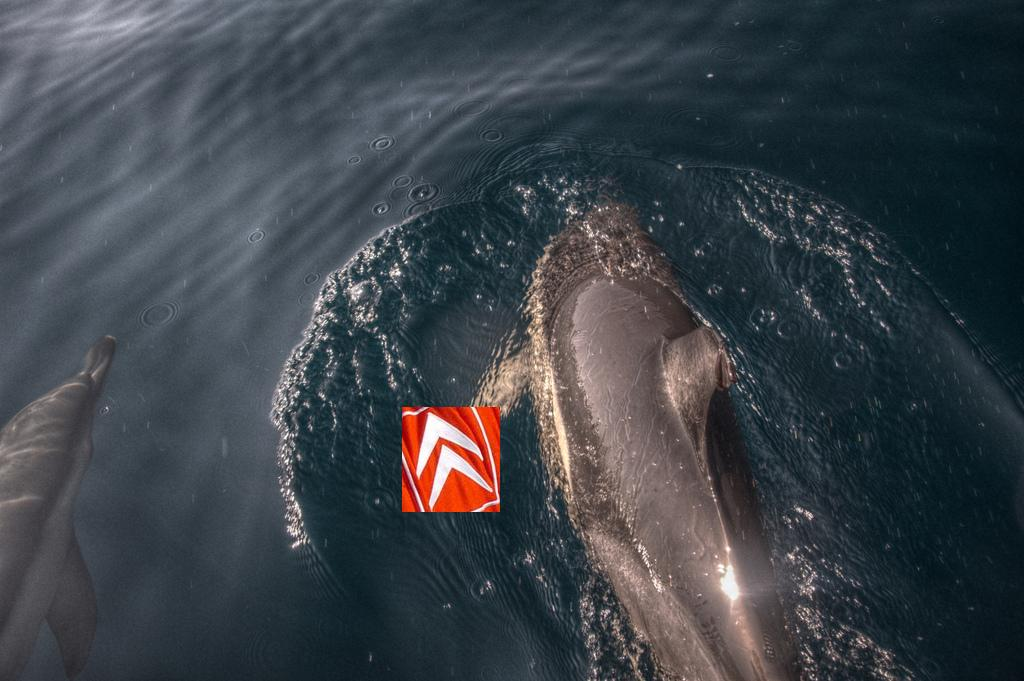
\includegraphics[width=25mm]{images/mt/flbl3.jpg} &   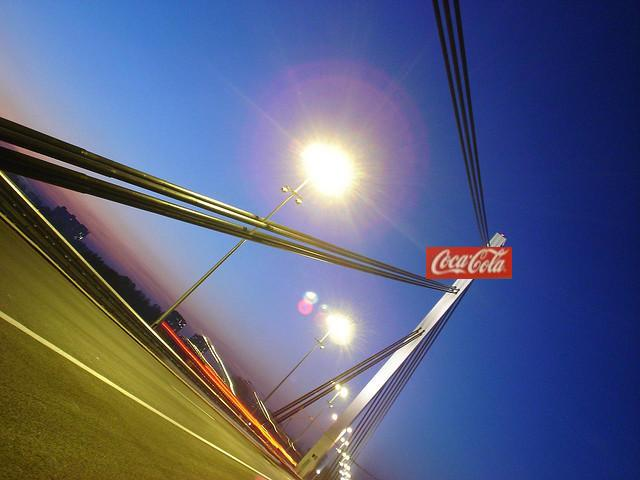
\includegraphics[width=25mm]{images/mt/flbl4.jpg} \\
    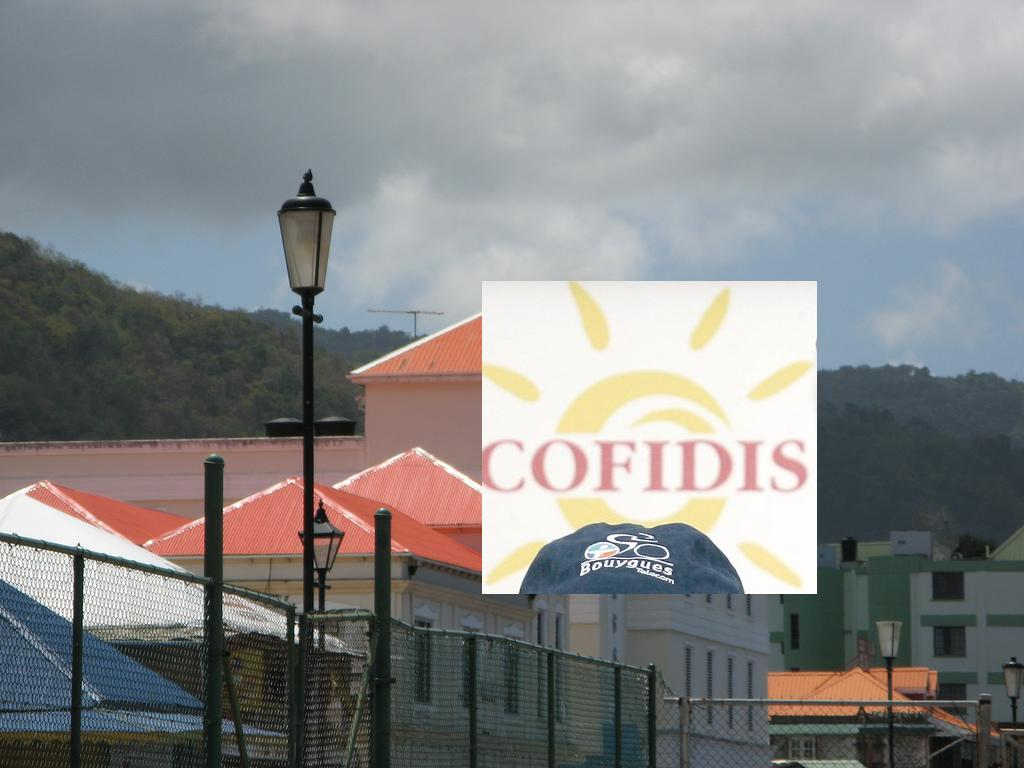
\includegraphics[width=25mm]{images/mt/flbl5.jpg} &   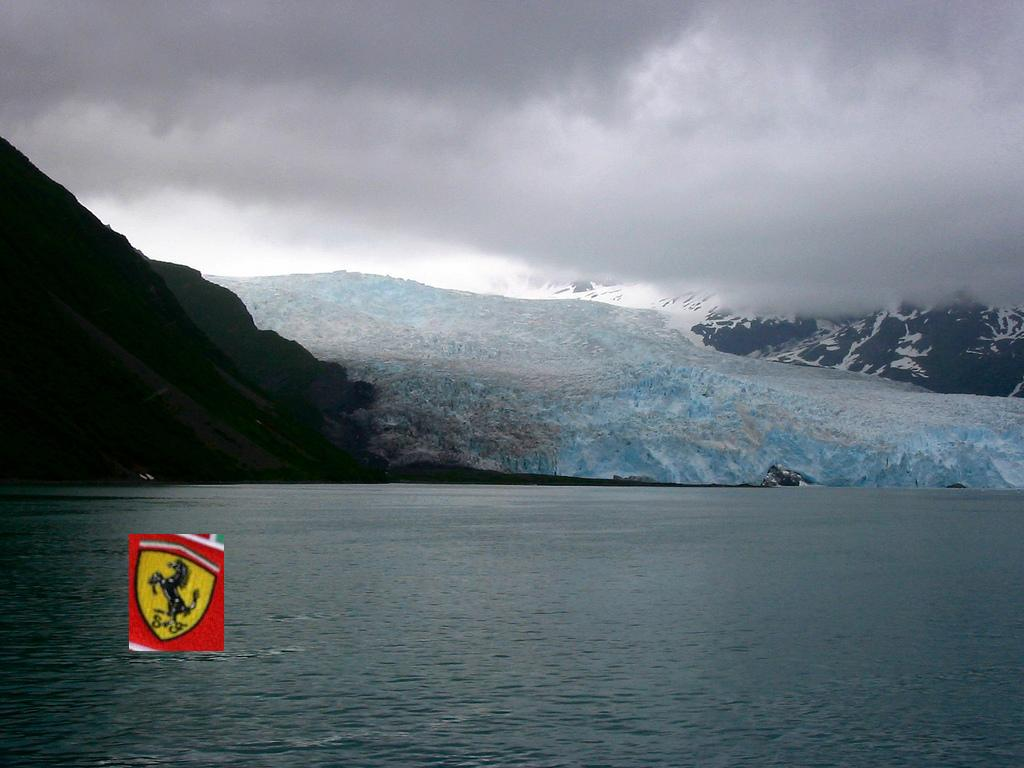
\includegraphics[width=25mm]{images/mt/flbl6.jpg}  & 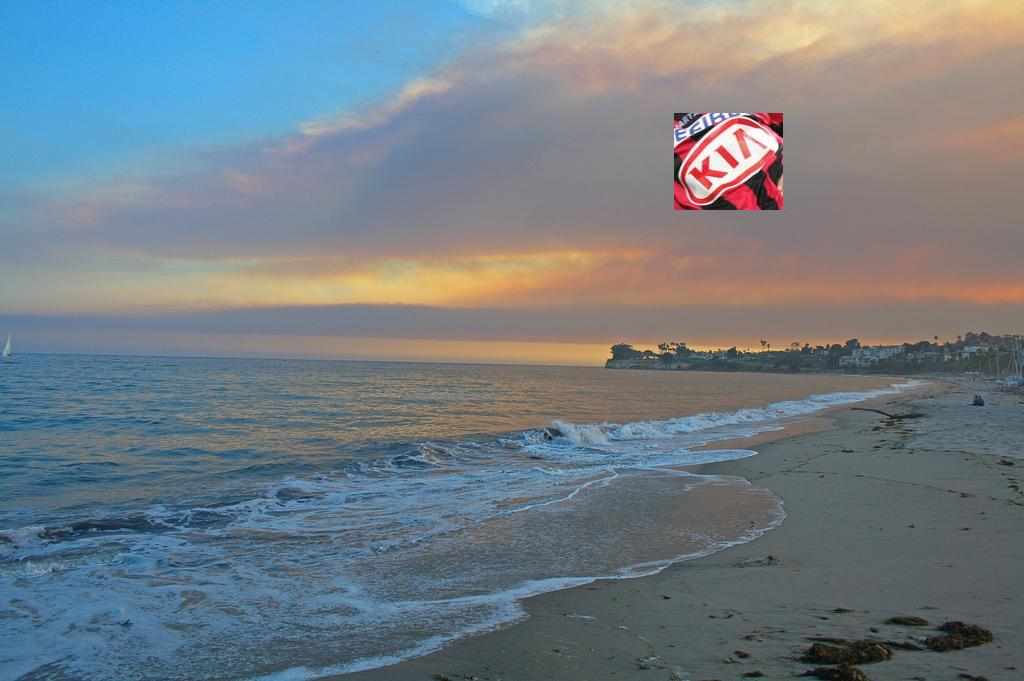
\includegraphics[width=25mm]{images/mt/flbl7.jpg} &   
\includegraphics[width=25mm]{images/mt/flbl8.jpg} 
\end{tabular}
\caption{FlickrBelgaLogos examples}
\end{figure}

This dataset was evaluated for training purposes. Therefore a small subset of BelgaLogos was chosen as test set. The logos on these images were leave out from the FlickrBelgaLogos dataset. The rest of the images is used as the train set to train a Faster R-CNN model with the 37 classes of BelgaLogos. The trained models are tested on the chosen test set of BelgaLogos. Then the train set of BelgaLogos was also trained with the same network, to compare the results. After that the datasets were fused to examine the possibility of achieving better performance. Lastly, the model was trained with curriculum learning \cite{Bengio_curriculumlearning} (CL) as it was done with logos in \cite{DBLP:journals/corr/SuZG16}. CL is a learning process, whereas the examples are gradually becoming more difficult during training. In this context, it is realized by training the network first merely with synthetic logos and then with real images.
\bigbreak
The synthetic dataset alone could achieve moderate results, the obvious advantage of a real dataset can be seen in figure \ref{f:flbltrain}. Unfortunately, the fusion of datasets does not bring extra performance, neither with a simply fusion, nor with curriculum learning. The latter has the advantage of achieving convergence much earlier, compared to other training scenarios. In \cite{DBLP:journals/corr/SuZG16}, 10\% relative extra performance was achieved by training with CL, to recognize a restricted number of classes. In case of FlickrBelgaLogos, this is probably not successful, because the same logos of BelgaLogos are reused in FlickrBelgaLogos. This means, while trying to achieve better performance, the transfer of logos to another context does not give additional information. As base network the \texttt{VGG\_CNN\_M} \cite{Chatfield14} was chosen, pretrained on ImageNet \cite{imagenet_cvpr09}, because of its much shorter training times, compared to VGG-16 (about a quarter as much time), still having a performance good enough for the experiments.
\bigbreak
The different points of the curves are collected by moving the decision boundary threshold on the scores of a region being object or not in the interval [0.01; 1), with 0.01.

\begin{figure}
  \centering
  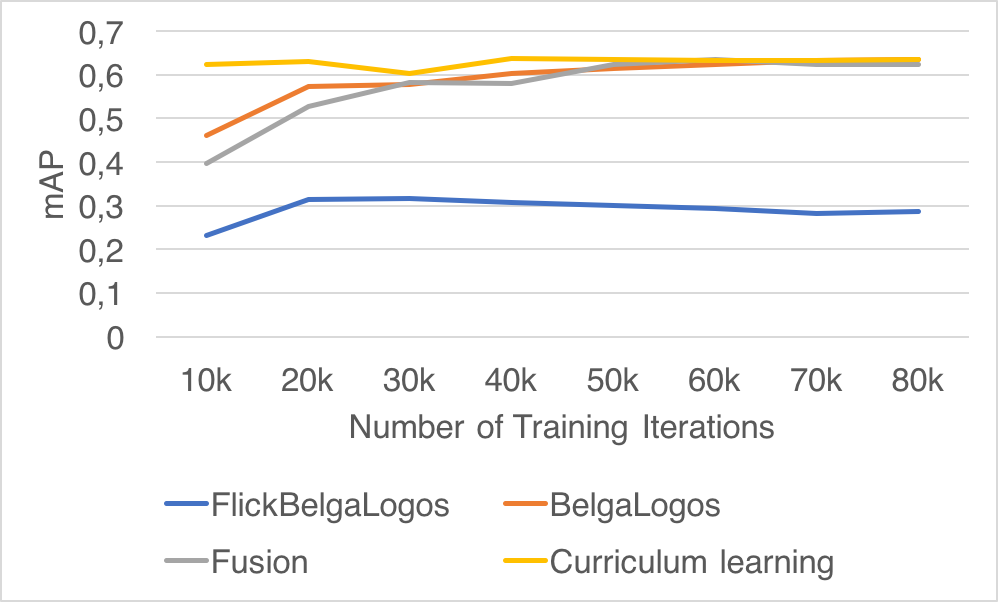
\includegraphics[width=80mm]{images/mt/flbl.png}
  \caption{Logo recognition performance after training with real (BelgaLogos) and synthetic data (FlickrBelgaLogos)}
  \label{f:flbltrain}
\end{figure}

After that, the open-set logo detection capability of the model, trained only on FlickrBelgaLogos, was tested. A faster R-CNN was trained purely for logo detection, without logo classes. For evaluation, a self annotated dataset of a sport video was used, that has logos merely from such companies, with which the net has not been trained before. Despite the small size and the unreality of this dataset, it is able to generalize from the learned logos and detect some of the logos unknown for the network. The detection performance evaluation can be seen in figure \ref{f:flbldeteval} as well as an example detection on \ref{f:flbldetexample}

\begin{figure}
  \centering
  \begin{tabular}{cc}
    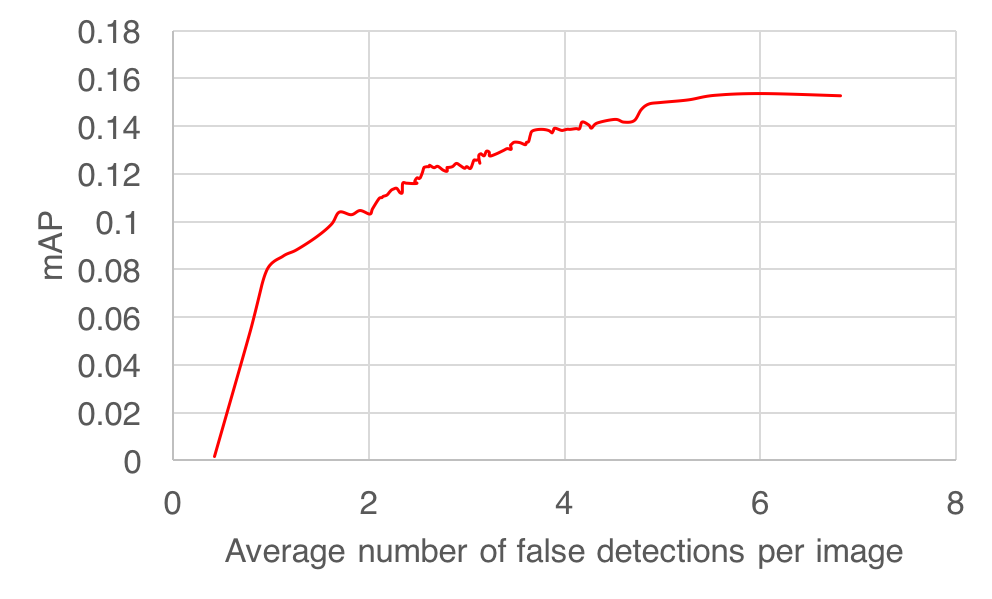
\includegraphics[width=80mm]{images/mt/flbl_det_map.png} & 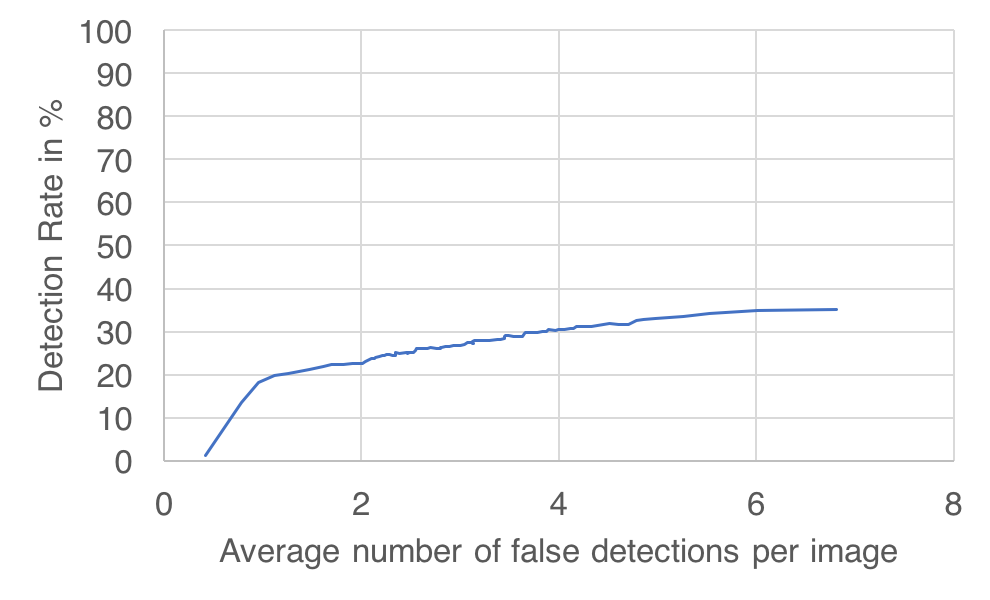
\includegraphics[width=80mm]{images/mt/flbl_det_froc.png}
  \end{tabular}
  \caption{Logo detection performance}
  \label{f:flbldeteval}
\end{figure}
\begin{figure}
  \centering
  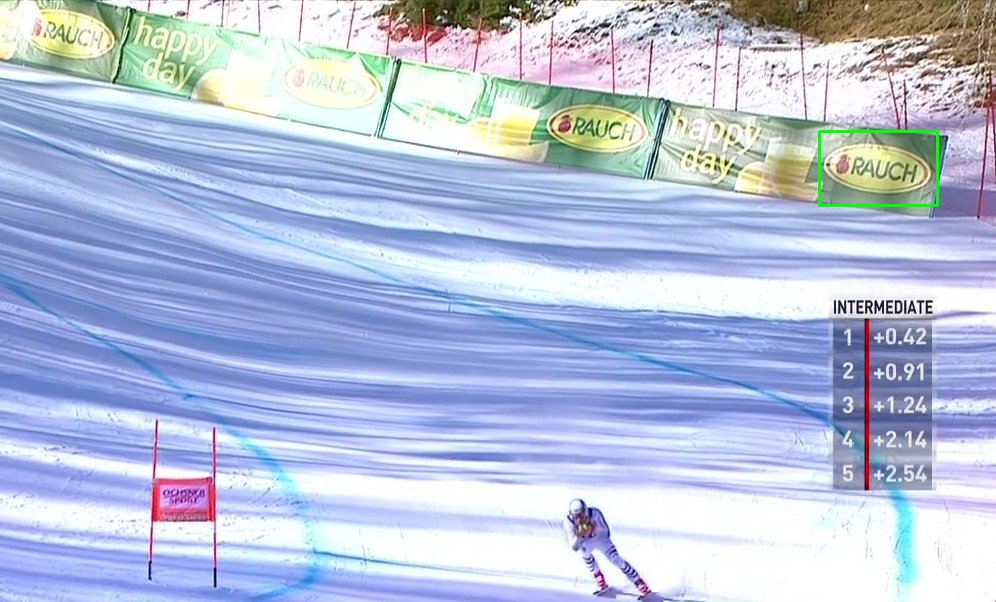
\includegraphics[width=80mm]{images/mt/flbl_det.png}
  \caption{Logo detection example}
  \label{f:flbldetexample}
\end{figure}
\bigbreak
\subsection{METU Trademark dataset}\label{ss:metu}

In order to extend the training dataset, a synthetic dataset was generated, where one logo from the METU Trademark dataset \cite{DBLP:journals/corr/TursunAK17} was placed on an image. As basis, photos from Tripadvisor were used to fulfill the requirement of being practically logo-free. The majority of the logo's background has a white color. But logos usually do have some background, other than white. Therefore some transformations were applied on the logo images before as follows. One third of the dataset was left unchanged. The brightness of the rest of them was adjusted to the brightness of the image, on which the logo is placed. Furthermore for one third of the logos, the mean HSV value of each logo was calculated and it was rotated with 90 degree chosen randomly. In addition, Gaussian blur was applied on the edges of the logos, in order to suppress the sharp contrast changes. The table \ref{table:logotransformations} summarizes the applied transformations.

\begin{table}[ht!]
\centering
\begin{tabular}{|c|c|c|}
\hline & \textbf{Brightness adjustment} & \textbf{Hue rotation} \\
\hline
\textbf{33\%} & - & - \\
\hline
\textbf{33\%} & yes & yes \\
\hline
\textbf{33\%} & yes & yes \\ \hline
\end{tabular}
\caption{Applied transformations}
\label{table:logotransformations}
\end{table}

The created dataset is then used to train a two class faster R-CNN for logo detection. The base network is again \texttt{VGG\_CNN\_M}, as in section \ref{ss:flickrbelgalogos}. For evaluation, the same self annotated sport video dataset was used, as in section \ref{ss:flickrbelgalogos}. Unfortunately, the trained network could not yield appropriate performance. The problem is probably that the dataset consists of logos mainly with a white background and a black text on them. The other source of problem could be the unreal appearance of the logos themselves or the transformations applied to them. Figure \ref{f:synmetu} shows some generated examples.

\begin{figure}
  \centering
  \begin{tabular}{cccc}
    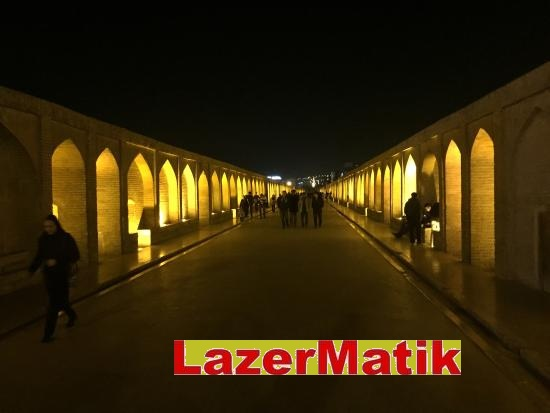
\includegraphics[height=20mm]{images/mt/synmetu1.jpg} &   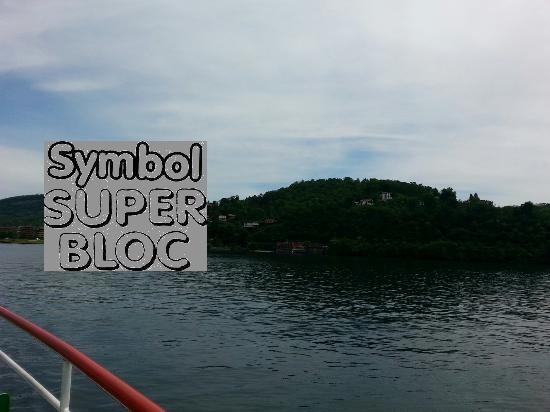
\includegraphics[height=20mm]{images/mt/synmetu2.jpg}  & 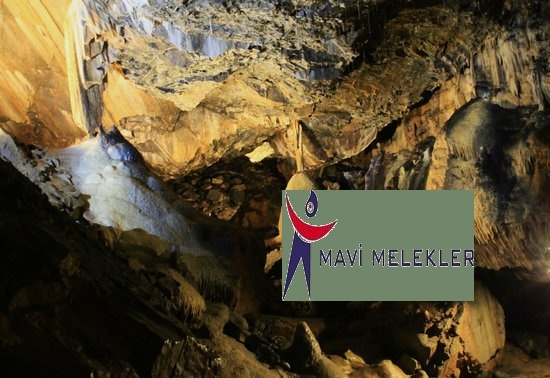
\includegraphics[height=20mm]{images/mt/synmetu3.jpg} &   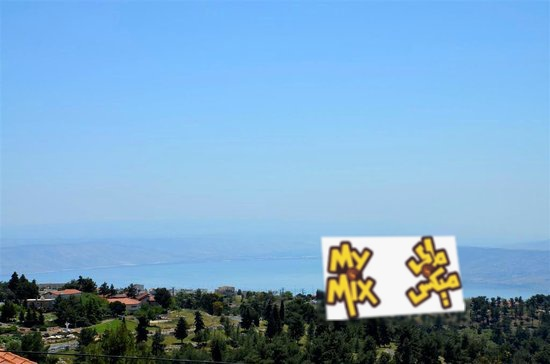
\includegraphics[height=20mm]{images/mt/synmetu4.jpg}\\
    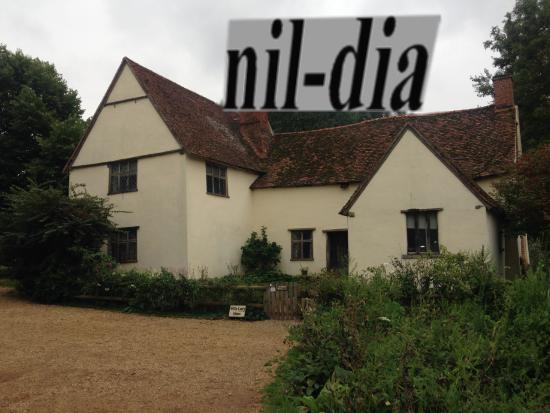
\includegraphics[height=20mm]{images/mt/synmetu5.jpg} &   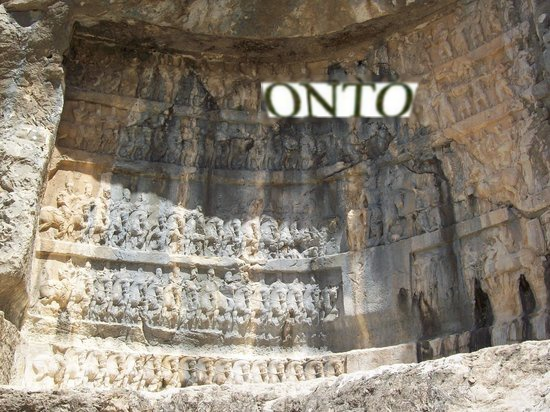
\includegraphics[height=20mm]{images/mt/synmetu6.jpg}  & 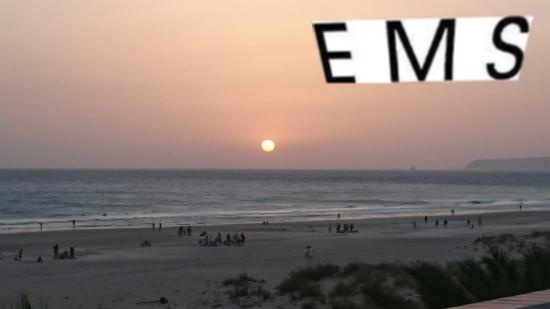
\includegraphics[height=20mm]{images/mt/synmetu7.jpg} &   
\includegraphics[height=20mm]{images/mt/synmetu8.jpg}
  \end{tabular}
  \caption{Generated synthetic logo images}
  \label{f:synmetu}
\end{figure}

\subsection{Synthetic data with shape based logos}

As section \ref{ss:metu} shows, the mainly text based logos are incapable to train a model to detect real logos. In order to successfully extend the training dataset, logo images with more shape and color \cite{LogoClearbit} were collected. The logos were simply copied and pasted to the same Tripadvisor dataset, as in section \ref{ss:metu}. Unfortunately, also this dataset was not able to train a model to generalize and to recognize real logos. As a next trial, the white background of the logos was set to transparent, as suggested in \cite{DBLP:journals/corr/SuZG16}, but in the context of open-set logo detection, it does not appear to be useful either. The success of FlickrBelgaLogos, seen in section \ref{ss:flickrbelgalogos}, was probably because the logo and its direct surrounding come from a real scene.
\bigbreak
\begin{figure}
  \centering
\begin{tabular}{cccc}
  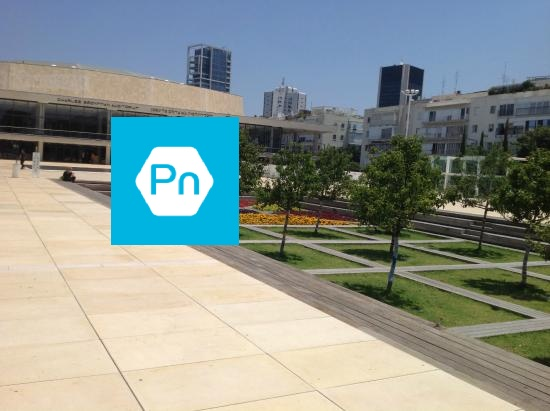
\includegraphics[height=20mm]{images/mt/clearbit1.jpg} &   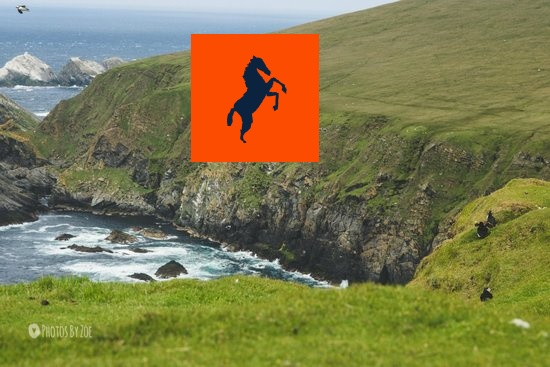
\includegraphics[height=20mm]{images/mt/clearbit2.jpg}  & 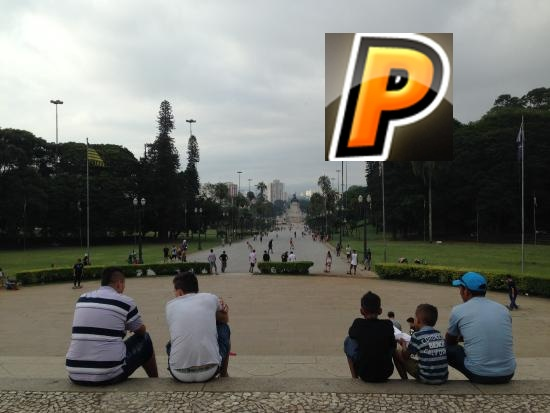
\includegraphics[height=20mm]{images/mt/clearbit3.jpg} &   
\includegraphics[height=20mm]{images/mt/clearbit4.jpg}
\end{tabular}
\caption{Generated synthetic logo images}
\label{f:synlogo}
\end{figure}
\bigbreak
\section{Logo Detection}\label{s:explogodetection}

Although there is not any known earlier work in the field of open-set logo detection and retrieval, it was still attempted to take a solution as baseline, which is already published. As section \ref{} details, there exists a lot of research in improving the retrieval performance on the FlickrLogos-32 dataset using faster R-CNN. Thereby, the region proposal network of a faster R-CNN is chosen for logo detector baseline, which is trained only on the train and validation set of FlickrLogos-32. The network itself achieves state-of-the-art performance on the test set of the dataset. In particular with VGG-16 as base network, it has 85.4 mAP, whereas the best already published result is 84.2 mAP proposed by \cite{Bao:2016:RCL:3007669.3007728}, using the multiscale fast R-CNN approach and AlexNet as base network.
\bigbreak
All the results of the following experiments are compared in figure \ref{f:detectioneval}. The data points are gathered by moving the threshold value on the region objectness probability emitted by the network.
Firstly, the RPN of the baseline network is evaluated on very challenging, self-annotated images, extracted from a football video. Afterwards, the network is trained on all the publicly available logo datasets with bounding box annotations, introduced in section \ref{s:logodatasets}, and the improvement of the RPN network is tested. This network has already a better recall performance, but it retrieves much more false locations for lower threshold values.
Next, a class agnostic faster R-CNN network is trained again on all public datasets, but now only with "logo" class. Both the RPN and the classifier with regression layer at the end of the network are tested. The latter output is referred as "FC" on the figure \ref{f:detectioneval}, because of the fully connected layers preceding them. A quite interesting result is here, that by training the same model with the same dataset without the specific brand labels, the performance of the region proposal network improves (see "Public Datasets RPN" versus "Public Datasets Class Agnostic RPN").

\begin{figure}
  \centering
  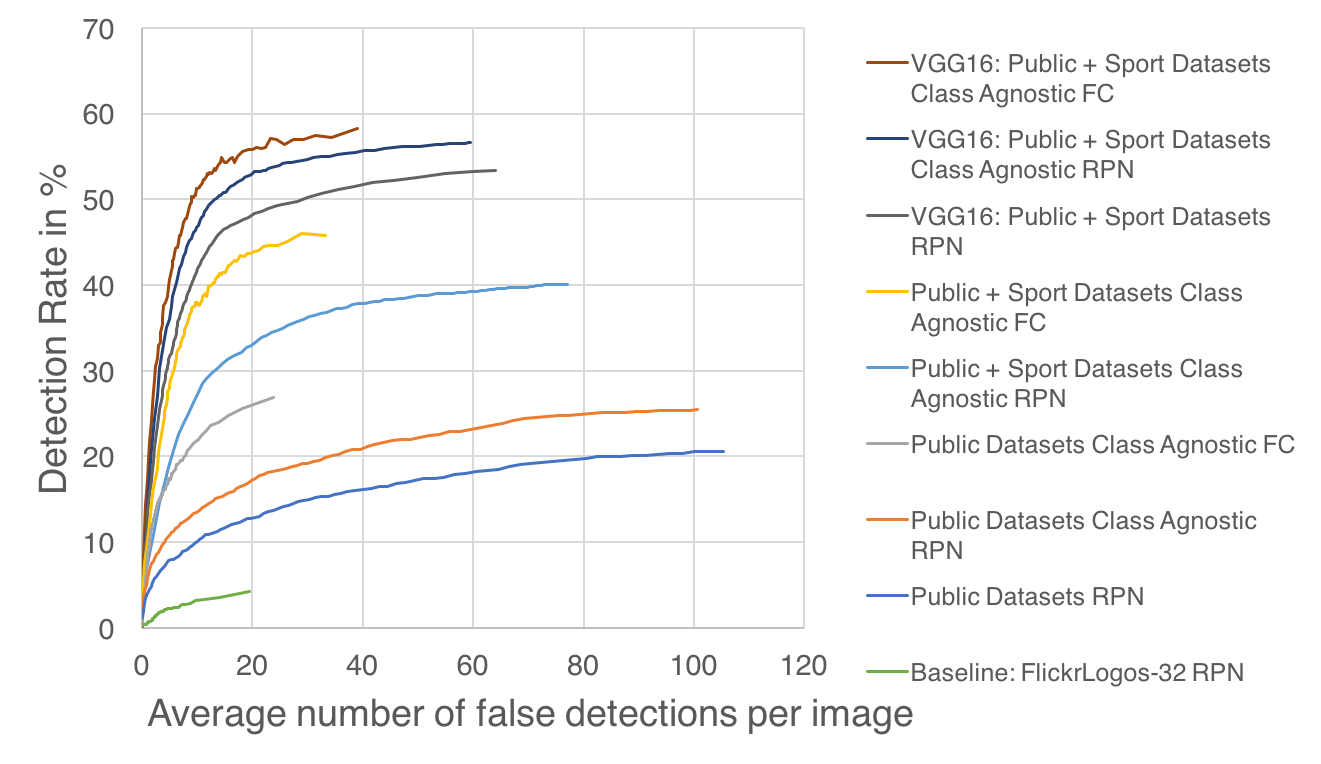
\includegraphics[width=120mm]{images/mt/logodetection.png}
  \caption{Logo detection evaluation}
  \label{f:detectioneval}
\end{figure}

In order to fine-tune the networks for the specific task, the datasets from similar context were used, introduced in section \ref{s:logodatasets}. The training is saturated after about one epoch learning. This means, that the initial network is good pretrained for the task. This data has a large effect on the performance.
\bigbreak
After training with so many logo brands, it is hard to find a sport video, with logos, which cannot be already found in the training set. E.g. Adidas is one of the brand, which occurs both in the training set and with a large number on the video. Nevertheless, the effect of that is questionable, because Adidas logos are coming from the datasets FlickrLogos-32 and Logos32Plus. The networks, trained already on these datasets achieve much weaker results.
\bigbreak
Finally, a VGG-16 based faster R-CNN was trained on all the training data, used earlier. Although, the gap between the RPN and the FC logo detector of this network became smaller, due to the much deeper base network, before the RPN, the FC solution yields still superior performance both in recall and precision. One could argue, that the marginal improvement of FC to RPN does not worth the increased computational complexity. However, the RPN network has about double as much false positive on the same level of recall. This can cause much more additional computational burden for the classifier, then what the FC layers do, especially if it needs large computational load.

The VGG-16 detector can generalize quite well, as figure \ref{f:extreme} shows it is able to operate under extreme light conditions too.

\begin{figure}
  \centering
  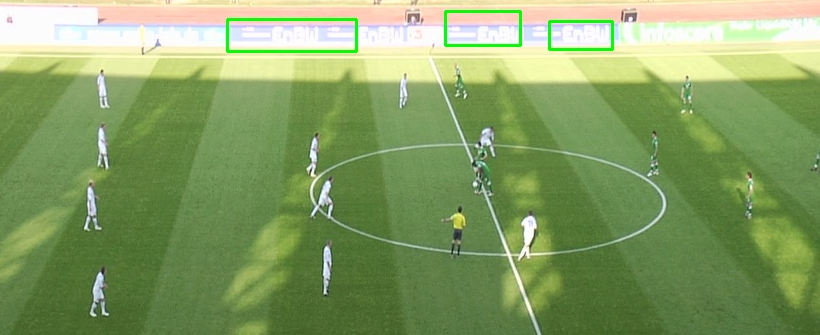
\includegraphics[width=120mm]{images/mt/extreme.png}
  \caption{Logo detection under extreme light conditions}
  \label{f:extreme}
\end{figure}

\section{Evaluation on FlickrLogos-32}
The effect of additional data and different architectures to the performance on the test set of FlickrLogos-32 (FL-32) is examined. The trained networks are the following ones:
\begin{enumerate}
    \item\label{i:first} A faster R-CNN, with \texttt{VGG\_CNN\_M\_1024} as base network, trained on the training and validation set of FL-32.
    \item\label{i:second} A jointly trained detector and classifier as introduced in section \ref{ss:solution4}, whereas the impact of further by training the classifier the same way as in point \ref{i:first}, and the detector on every other public datasets without specific brand label.
    \item\label{i:third} A faster R-CNN is trained, based on \texttt{VGG\_CNN\_M\_1024}, trained on the same datasets as the detector and classifier together in point \ref{i:second}, but this time with complete brand specification.
    \item Point \ref{i:first} and \ref{i:second} is repeated with VGG-16
    \item A faster R-CNN, trained on all public datasets, and annotated sport videos
\end{enumerate}

The test set of FL-32 is evaluated with the configurations from points \ref{i:first}, \ref{i:second} and \ref{i:third}, and compared in figure \ref{f:vggcnnmfltest}. The networks are evaluated based on the mAP. It can be seen, that additional logo dataset, even without brand indication can be utilized, to detect and recognize known logos with better performance, by using the Siamese-like architecture, proposed in \ref{ss:solution4}. The network, trained on complete class information starts with a worse performance. It is because of the more number of iterations, needed to be able to distinguish between the much more learned classes. Later on, it has obviously superior performance.

\begin{figure}
  \centering
  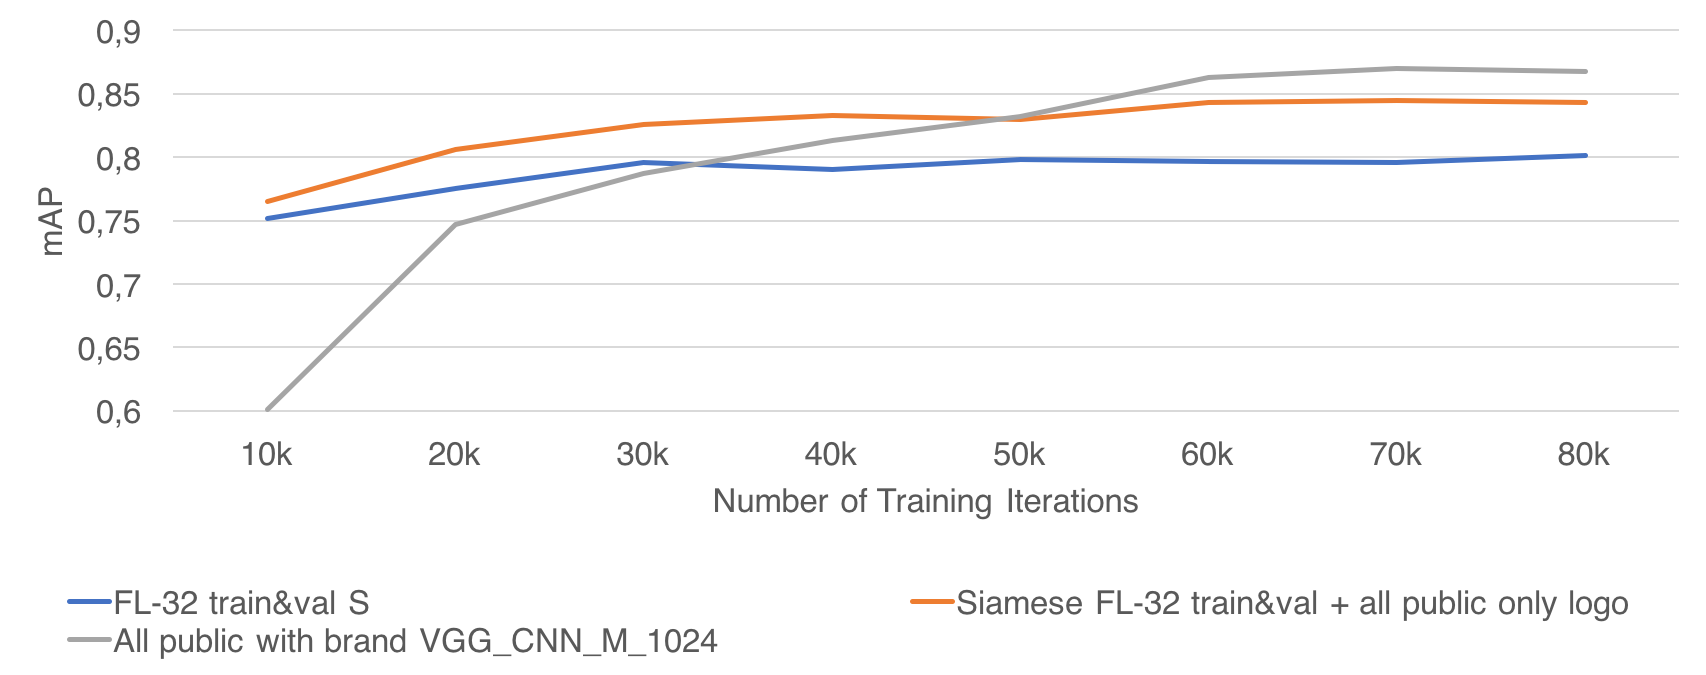
\includegraphics[width=120mm]{images/mt/vggcnnmfltest.png}
  \caption{FL-32 test evaluation with \texttt{VGG\_CNN\_M\_1024} base network}
  \label{f:extreme}
\end{figure}

The improvement of additional data on the performance is then tested with VGG16 base network, having more capacity. Due to the more data, it achieves naturally state-of the-art performance on FL-32 test set.

\section{Logo Retrieval}

After the best logo detector is found, the system should decide, which detections are relevant, and classify them, to the instances of the query set.

As a baseline system for logo retrieval, the solution detailed in section \ref{ss:solution1} was chosen, because this system holds the state-of-the-art performance in closed set logo retrieval. It consists of a faster R-CNN, trained for logo detection on the train and validation set of FL-32.
\bigbreak
As detailed in section \ref{ss:solution1}, this solution may have a hard time detecting the complete logo, especially if the logo has more distinct parts. The effect of mislocalization and the low number of output features probabilities of the last layer is further investigated. To this end, the performance of the class probabilities was qualitatively tested. In particular, three logo images were tested from the same, unknown brand, having lesser or greater appearance variation:
\begin{itemize}
	\item a logo, cropped from a video
	\item a logo with very similar background color, but in high resolution
	\item a logo with a completely different color scheme also in high resolution
\end{itemize}

The logos fill out the majority of the images as figure \ref{} shows. The assumption was, that despite the unknownness of the brand, the descriptor features of the three logos will contain similar portion of probabilities of known brands, thus having low cosine distance to each other. Unfortunately, the network was incapable to yield such feature vectors, the logos and the associated logo from the known set with the greatest probability can be seen in figure \ref{f:confusion}. The composition of the normed features for the three query images is shown by figure \ref{}

\begin{figure}
  \centering
  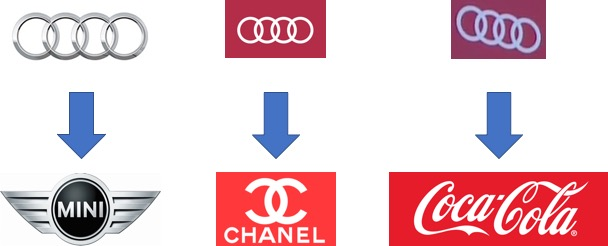
\includegraphics[height=40mm]{images/mt/confusion.jpg}
  \caption{}
  \label{f:fasterconfusion}
\end{figure}

\begin{figure}
  \centering
  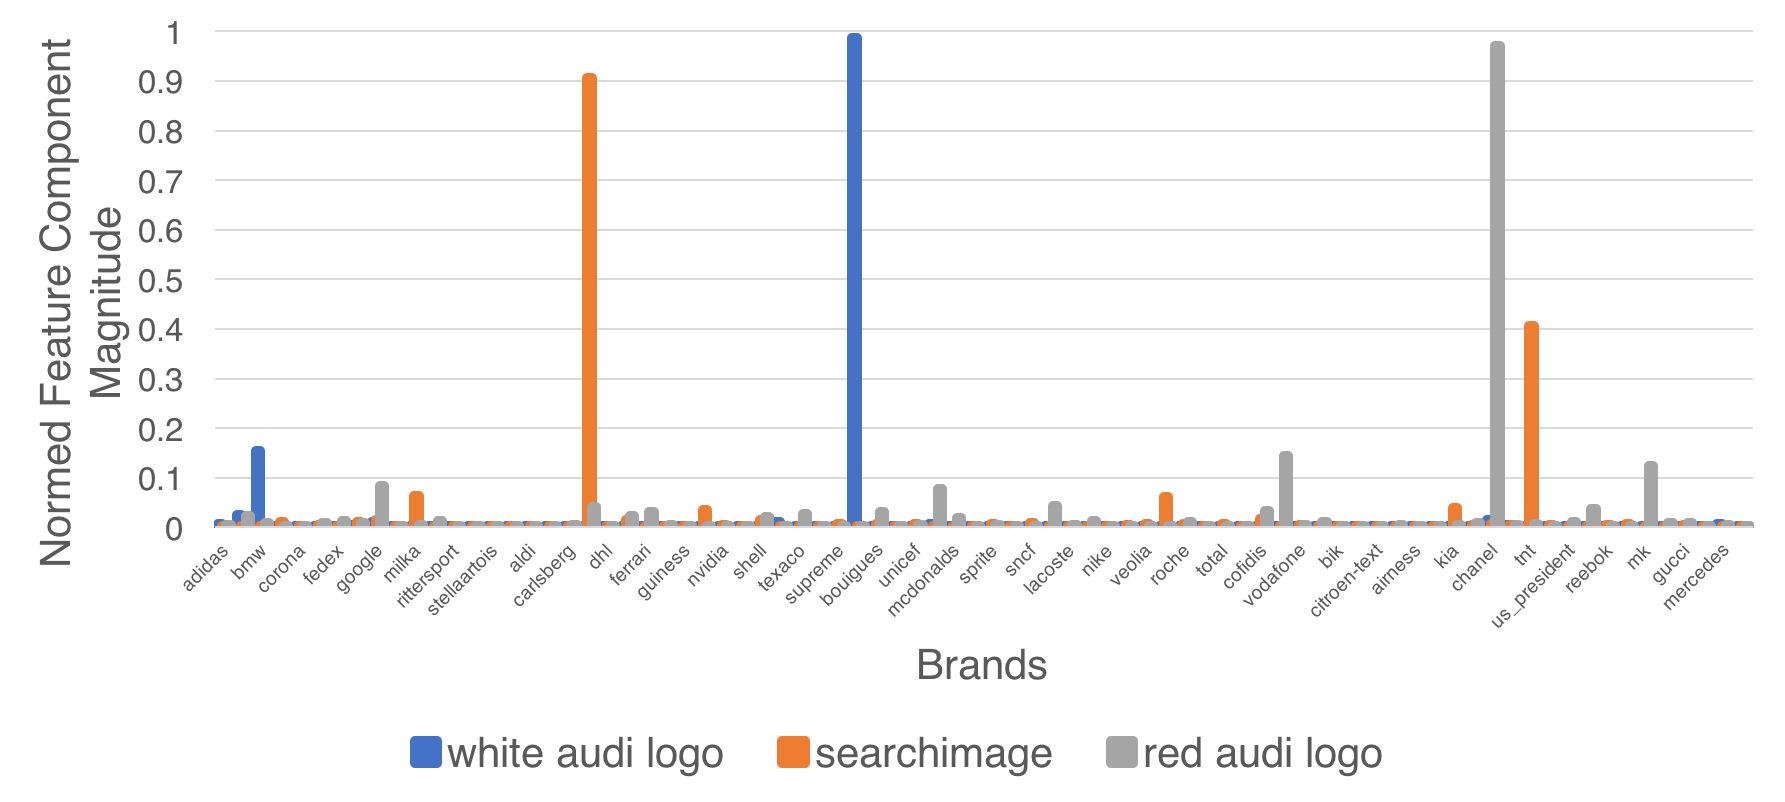
\includegraphics[height=80mm]{images/mt/faster_confusion.png}
  \caption{}
  \label{f:confusion}
\end{figure}

Joint 


General convnets
The proposed bounding box regions are warped to 224x244 pixels, which is the conventional input size of these networks. No padding were used for the crops, so the aspect ratio was not preserved. This should not induce errors, because the query images undergo this aspect ratio change too.

The retrieval performance was then tested, with query images, cropped from the video. But because of the are large intraclass variances it still a challenging task for the classifier. Figure \ref{f:largevar} shows groundtruth examples.

\begin{figure}
  \centering
    \begin{tabular}{cccc}
      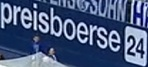
\includegraphics[width=25mm]{images/mt/largevar_1_b.jpg} &   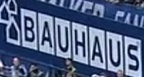
\includegraphics[width=25mm]{images/mt/largevar_2_a.jpg}  & 
\includegraphics[width=25mm]{images/mt/largevar_3_a.jpg} &   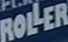
\includegraphics[width=25mm]{images/mt/largevar_4_a.jpg} \\
      
\includegraphics[width=25mm]{images/mt/largevar_1_a.jpg} &   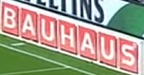
\includegraphics[width=25mm]{images/mt/largevar_2_b.jpg}  & 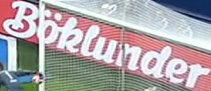
\includegraphics[width=25mm]{images/mt/largevar_3_b.jpg} &   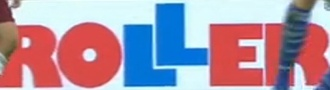
\includegraphics[width=25mm]{images/mt/largevar_4_b.jpg}
    \end{tabular}
  \caption{Samples for intraclass variation in one sport video. Images from same columns have the same class.}
  \label{f:largevar}
\end{figure}
Occluded images are not included in the test set, because perhaps neither a TV-viewer would find the correspondence for unknown logos. Images, which have an edge size both in width and height smaller or equal than 25 pixel are also omitted, because those escape the viewer's attention too very likely. In addition, classes, having only one example were removed, because in this case the query set would cover the groundtruth.

The similarities between the extracted feature vectors were calculated by cosine distance. 

Audi logo crop classification highres, crop, white



Classification performance by chance

\section{Retrieval times}